\documentclass[convert]{article}		
\usepackage{etex}
\usepackage[pdftex]{graphicx}
\usepackage{xcolor}
%\input{preambule}
%\usepackage{graphicx}
\usepackage{qrcode}
\usepackage{fix-cm}
\pagestyle{empty} 

% fond d'écran
\usepackage{eso-pic}
\newcommand\BackgroundA{%
	\put(0,0){%
		\parbox[b][\paperheight]{\paperwidth}{%
			\vfill
			\centering
			\includegraphics[width=\paperwidth,height=\paperheight,%
			keepaspectratio]{../../media/@fondDiplome@}%
			\vfill
}}}


\usepackage[a5paper,landscape]{geometry}
\geometry{right=0.5cm,left=0.5cm,top=1cm,bottom=1cm}

% pour le surlignement en gras
%\usepackage{mathtools}
%\newcommand*{\myov}[1]{\overbracket[3.65pt][0pt]{#1}}
%\newcommand*{\myovline}[2]{\overbracket[#2][-1pt]{#1}}
\usepackage[usestackEOL]{stackengine}
\usepackage{scalerel}
\def\myoverline#1{\ThisStyle{%
		\setbox0=\hbox{$\SavedStyle#1$}%
		\stackengine{7\LMpt}{$\SavedStyle#1$}{\rule{\wd0}{4\LMpt}}{O}{c}{F}{F}{S}%
}}

\begin{document}
\AddToShipoutPicture*{\BackgroundA}

\color{white}

{\Huge\textbf{@intituleCross@ @lieu@}}

\bigskip

\resizebox{!}{40pt}{@nomCourse@}

\bigskip

{\Huge \textbf{@date@}}

\vfill

%\begin{minipage}[c]{6cm}
\resizebox{!}{40pt}{\textbf{@rang@ème} 	} {\Huge / @nbreTotal@ participants}

\bigskip
%\end{minipage}
%\begin{minipage}[c]{18cm}
\textbf{\Huge @nom@ @prenom@}

\bigskip

\textbf{\huge @categorie@ : @rangCat@ / @nbreTotalCategorie@}
	
%\textbf{}
%\end{minipage}
\bigskip


\begin{minipage}[c]{1.5cm}
	
\includegraphics[width=\textwidth]{../../media/chronometre-blanc.png}
\end{minipage}
\begin{minipage}[c]{4cm}
	\textbf{\huge @temps@}
\end{minipage}
%\hspace{0.5cm}
\hfill
\begin{minipage}[c]{1.5cm}
	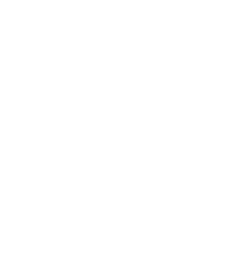
\includegraphics[width=\textwidth]{../../media/vitesse-blanc.png}
\end{minipage}
\begin{minipage}[c]{4cm}
	\textbf{\huge @vitesse@}
\end{minipage}
%\hspace{0.5cm}
\hfill
\begin{minipage}[c]{1cm}
	\includegraphics[width=\textwidth]{../../media/@logoSexe@}
\end{minipage}
\begin{minipage}[c]{5cm}
	\textbf{\huge @rangSexe@ème / @nbreTotalSexe@}
\end{minipage}

\end{document}
